\chapter{Basic RDE Scheme}
\label{ch:basic-rde-scheme}

In this chapter we further explain the basic RDE scheme presented in~\cite{verheul2017remote}.

We distinguish three phases in the RDE scheme: (1) enrollment, (2) key generation, and (3) decryption (or key retrieval).
In the enrollment phase, the user (recipient) enrolls their passport for usage with RDE by extracting some data from the passport.
This is done by using a reader app that can communicate with the passport via NFC.
Enrollment results in certain \textit{enrollment parameters}, which one could consider as some sort of RDE public key of the user.
We will however not use the term public key further, as this could be confusing with actual the public key of the password that is included in the enrollment data.
We rather use the term \textit{enrollment parameters}.

In the key generation phase, someone (the sender) retrieves the \textit{enrollment parameters} and generates an RDE key pair for the recipient.
This results in a \textit{secret key}, and \textit{decryption parameters}.
The \textit{secret key} can be used to do the actual encryption of the message or files.
The \textit{decryption parameters} need to be sent back to the recipient, together with the encrypted message or files and does not need to be kept secret.
During decryption, the recipient uses the \textit{decryption parameters} together with their passport to retrieve the secret key and actually decrypt the message or files.

A high-level overview of this scheme is shown in Figure~\ref{fig:basic-rde-scheme}.
\begin{figure}
\centering
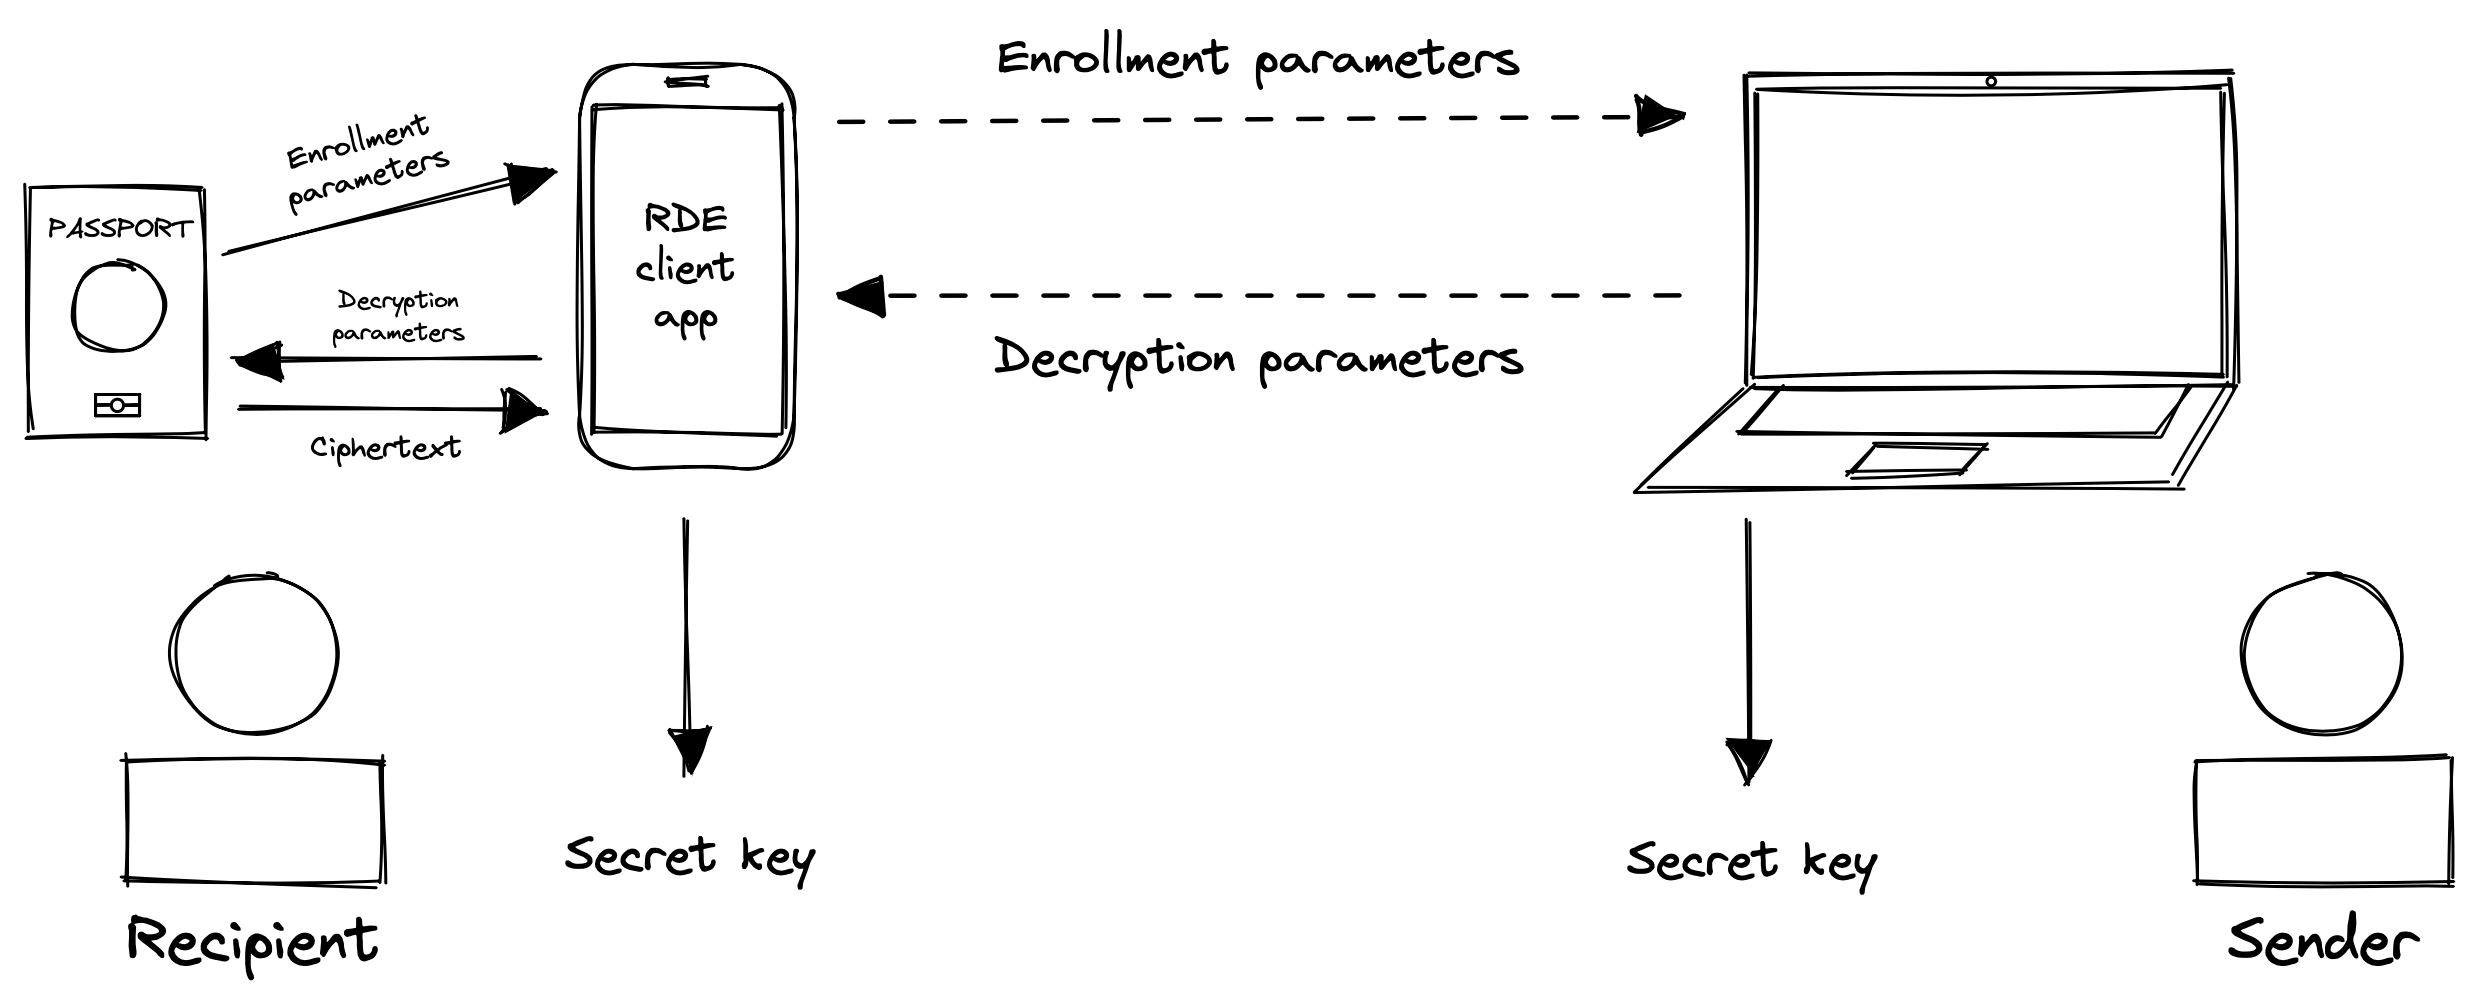
\includegraphics[width=0.8\textwidth]{imgs/RDE overview}
\caption{High-level overview of the basic RDE scheme.}
\label{fig:basic-rde-scheme}
\end{figure}

\section{E-passports}
\label{sec:e-passports}
E-passports are electronic passports that function as a smart card.
They contain a chip that can store data and execute programs.
Data on e-passports is stored in files, called Elementary Files (EFs) containing certain Data Groups (DGs).
For our report the most interesting files on the passport for RDE are the DG1, DG2, DG14, and EFsod.
\begin{itemize}
    \item DG1 contains the personal data of the holder of the passport.
    This group contains the information that is also printed on the passport itself in the machine-readable zone (MRZ).
    The data in this group is thus also referred to as the MRZ data.
    \item DG2 contains the facial image of the holder of the passport.
    \item DG14 contains security info of the passport.
    Most notably, it contains the Chip Authentication (CA) public key of the passport
    \item The EFsod contains the security object data of the passport.
    It contains a hash of all data groups on the passport, as well as a certificate from the country that issued the passport.
    The certificate can be used to verify the authenticity of the data.
\end{itemize}

\subsection{Secure messaging (BAC and PACE)}\label{subsec:secure-messaging}
Readers can communicate with an e-passport at different levels of security.
The most basic level is plain messaging and does not provide any security features.
At this level, the passport will not respond to any commands, except for querying the supported security levels and initiating a secure messaging session.
In order to actually communicate with the passport, a secure messaging channel must be set up.
Currently, there are two ways to set up a secure messaging channel: Basic Access Control (BAC) and Password Authenticated Connection Establishment (PACE).

\subsubsection{Basic Access Control (BAC)}\label{subsubsec:basic-access-control}
BAC works via a challenge response mechanism, where the reader requests a random challenge from the passport, and then shows knowledge of the BAC key by properly responding to this challenge.
The key is based on three fields from the MRZ: the date of birth, the date of expiry, and the document number.
After BAC, further communication with the passport is encrypted using the 3DES algorithm.

\subsubsection{Password Authenticated Connection Establishment (PACE)}\label{subsubsec:password-authenticated-connection-establishment}
A second and more modern way for this first level of security is Password Authenticated Connection Establishment (PACE).
PACE first performs a (Elliptic Curve) Diffie-Hellman key exchange to generate a session key, which is then used to encrypt the communication.
Authentication is then still done with the BAC key derived from the MRZ data (or on certain passports, with the Card Access Number (CAN) that is printed on the passport).
According to the ICAO standard, PACE is the preferred method for setting up a secure messaging channel as it is more secure than BAC.
BAC should only be used as fallback when PACE is not supported by the passport~\cite{icao9303securitymechanisms}.
Note that on the most recent Dutch passports, BAC is no longer supported and PACE must be used for the first level of security.


BAC and PACE do not provide any real authentication of the document itself or the document holder.
They only prevent eavesdropping on the communication between the reader and the passport and prevent skimming attacks (where an attacker reads data from the passport without the user noticing, for example when walking through an airport).
Using the BAC key (or CAN) requires the reader of the passport to actually have physical access to the passport (or at least the MRZ data).

\subsection{Passive Authentication (PA)}\label{subsec:passive-authentication}
After the first level of security has been established, the reader can read data from the document.
To authenticate whether this data actually belongs to a valid passport, the reader can perform passive authentication.
This requires the contents of the EFsod file to be read from the passport.
The reader can calculate the hashes of the data groups on the passport and compare them to the hashes in the EFsod file.
Additionally, it should verify the authenticity of the read EFsod file by checking a hash on those contents, and verifying the signature on the file.
This signature is created using the public key of the country that issued the passport, the so-called \textit{document signing key}.
Finally, the certificate chain should be verified.
This ultimately requires the reader to have a trusted list of document signing keys.
There are several ways to obtain such list, for example by downloading it from the ICAO website, or from a country's public key directory.

Note that the steps above are all be performed by the reader and do not require any processing capabilities on the passport itself.
This is why these steps are called passive authentication: the passport does not actively participate in the authentication process.

\subsection{Chip Authentication (CA)}\label{subsec:chip-authentication}
The aforementioned passive authentication only verifies the authenticity of data on the passport, but does not verify if the data is actually from the physical passport that is presented.
We could also be dealing with a fake passport that is replaying the data from a real passport.
In order to verify that the passport is actually the passport that is presented, the passport needs to actively participate in an authentication protocol.
This can be done via different protocols: by Active Authentication (AA) or Chip Authentication (CA).
For RDE, we use only use the latter.

Chip Authentication (CA) is a protocol that uses the CA public key of the passport to authenticate the passport.
This key is stored in the DG14 file on the passport.
Upon perform CA, (Elliptic Curve) Diffie-Hellman is performed between the passport and the reader.
The shared secret of this handshake is then used for further communication in the session.
Note that this replaces the keys that were set up earlier with BAC or PACE.

Note that with CA, the passport proofs it has access to the private key that belongs to the CA public key (which in its turn is signed by the government via the EFsod).
This is how we know that we are communicating with the real passport and not a fake passport that is replaying.

Note that according to the ICAO standards, CA does not necessarily need to be ECDH, but can also be RSA-based.
However, in practice, ECDH is used more often.
We will use the term ECDH in the rest of this report, but note that RSA-based DH also works.

\subsection{Terminal Authentication (TA)}\label{subsec:terminal-authentication}
For completeness, we also briefly mention Terminal Authentication (TA).
With TA, the reader proves to the passport that it is a trusted reader, via a challenge-response mechanism.
This is required for some applications.
For example, in order to read certain biometric data from the passport, like fingerprints, the reader must prove to the passport that it is a trusted reader.
For RDE, we do not use TA.

\section{RDE basic idea}\label{sec:rde-basic-idea}
When performing the CA ECDH key exchange step, the passport will always use the same key for its part of the handshake: it uses the public key that is stored in the DG14 file.
After CA, further communication is encrypted using keys deterministically derived from the shared secret of the ECDH key exchange.
This means that the freshness of the communication, relies on the freshness of the ephemeral key chosen by the reader.

After CA, when the reader tries to read the data on the passport, the passport will respond with a ciphertext that is encrypted using the keys derived from the shared secret.
Because strong encryption is used, the data will look random to anyone not in possession of this shared secret.
Everytime a reader chooses the same ephemeral key for its part in the ECDH key exchange, the same shared secret will be generated, and reading this data group will result in the same ciphertext.
RDE is based on this idea.

\begin{enumerate}
    \item Upon enrollment, we read the CA public key of the passport (after having performed BAC or PACE).
    We also read the contents of one of the data groups on the passport.
    This can be any data group that can be read without TA.
    In most cases, this will be DG14 as this data group does not contain any privacy-sensitive data and is of sufficient size to return long enough ciphertexts later.
    \item During RDE key generation, we retrieve this information and choose our own ephemeral key that is compatible with the CA public key of the passport.
    We simulate ECDH with the CA public key of the passport (that is included in the enrollment parameters) and compute the shared secret.
    We then use this shared secret and the derived keys to emulate how the passport would reply to us when we would try to read the contents of the chosen data group (from which we know the plaintext from the enrollment parameters).
    This emulated ciphertext response will be used to construct the secret key.
    Furthermore, we also need to emulate, using the shared secret and the derived keys, what our encrypted read command should look like if we were to actually communicate with the passport.
    The emulated encrypted read command (also referred to as protected command), together with the public key we chose ourselves, together form the RDE decryption parameters.
    \item When as recipient, we want to retrieve the secret message key, we use the provided RDE decryption parameters.
    First we perform BAC or PACE to set up the first level of security.
    Then we perform the ECDH with the provided public key from decryption parameters (that was chosen by the sender).
    Even though we as recipient do not know the shared secret our passport is using (as we do not have the private key the sender generated), the passport will know this shared secret (as it is based on the private key that is securely stored on the passport).
    We then send the protected command to the passport.
    The passport will be able to decrypt this command, and then reply with the encrypted contents of the chosen data group.
    This will match the ciphertext response that was emulated by the sender.
    The reader then derives the secret key from this ciphertext response.
\end{enumerate}

For deriving the secret key from the ciphertext response, we simply take a hash of the ciphertext.

For further details on the RDE protocol, we refer to the explanation provided in~\cite{verheul2017remote}.
A schematic of the decryption process is shown in Figure~\ref{fig:rde-decryption}.
\begin{figure}
    \centering
    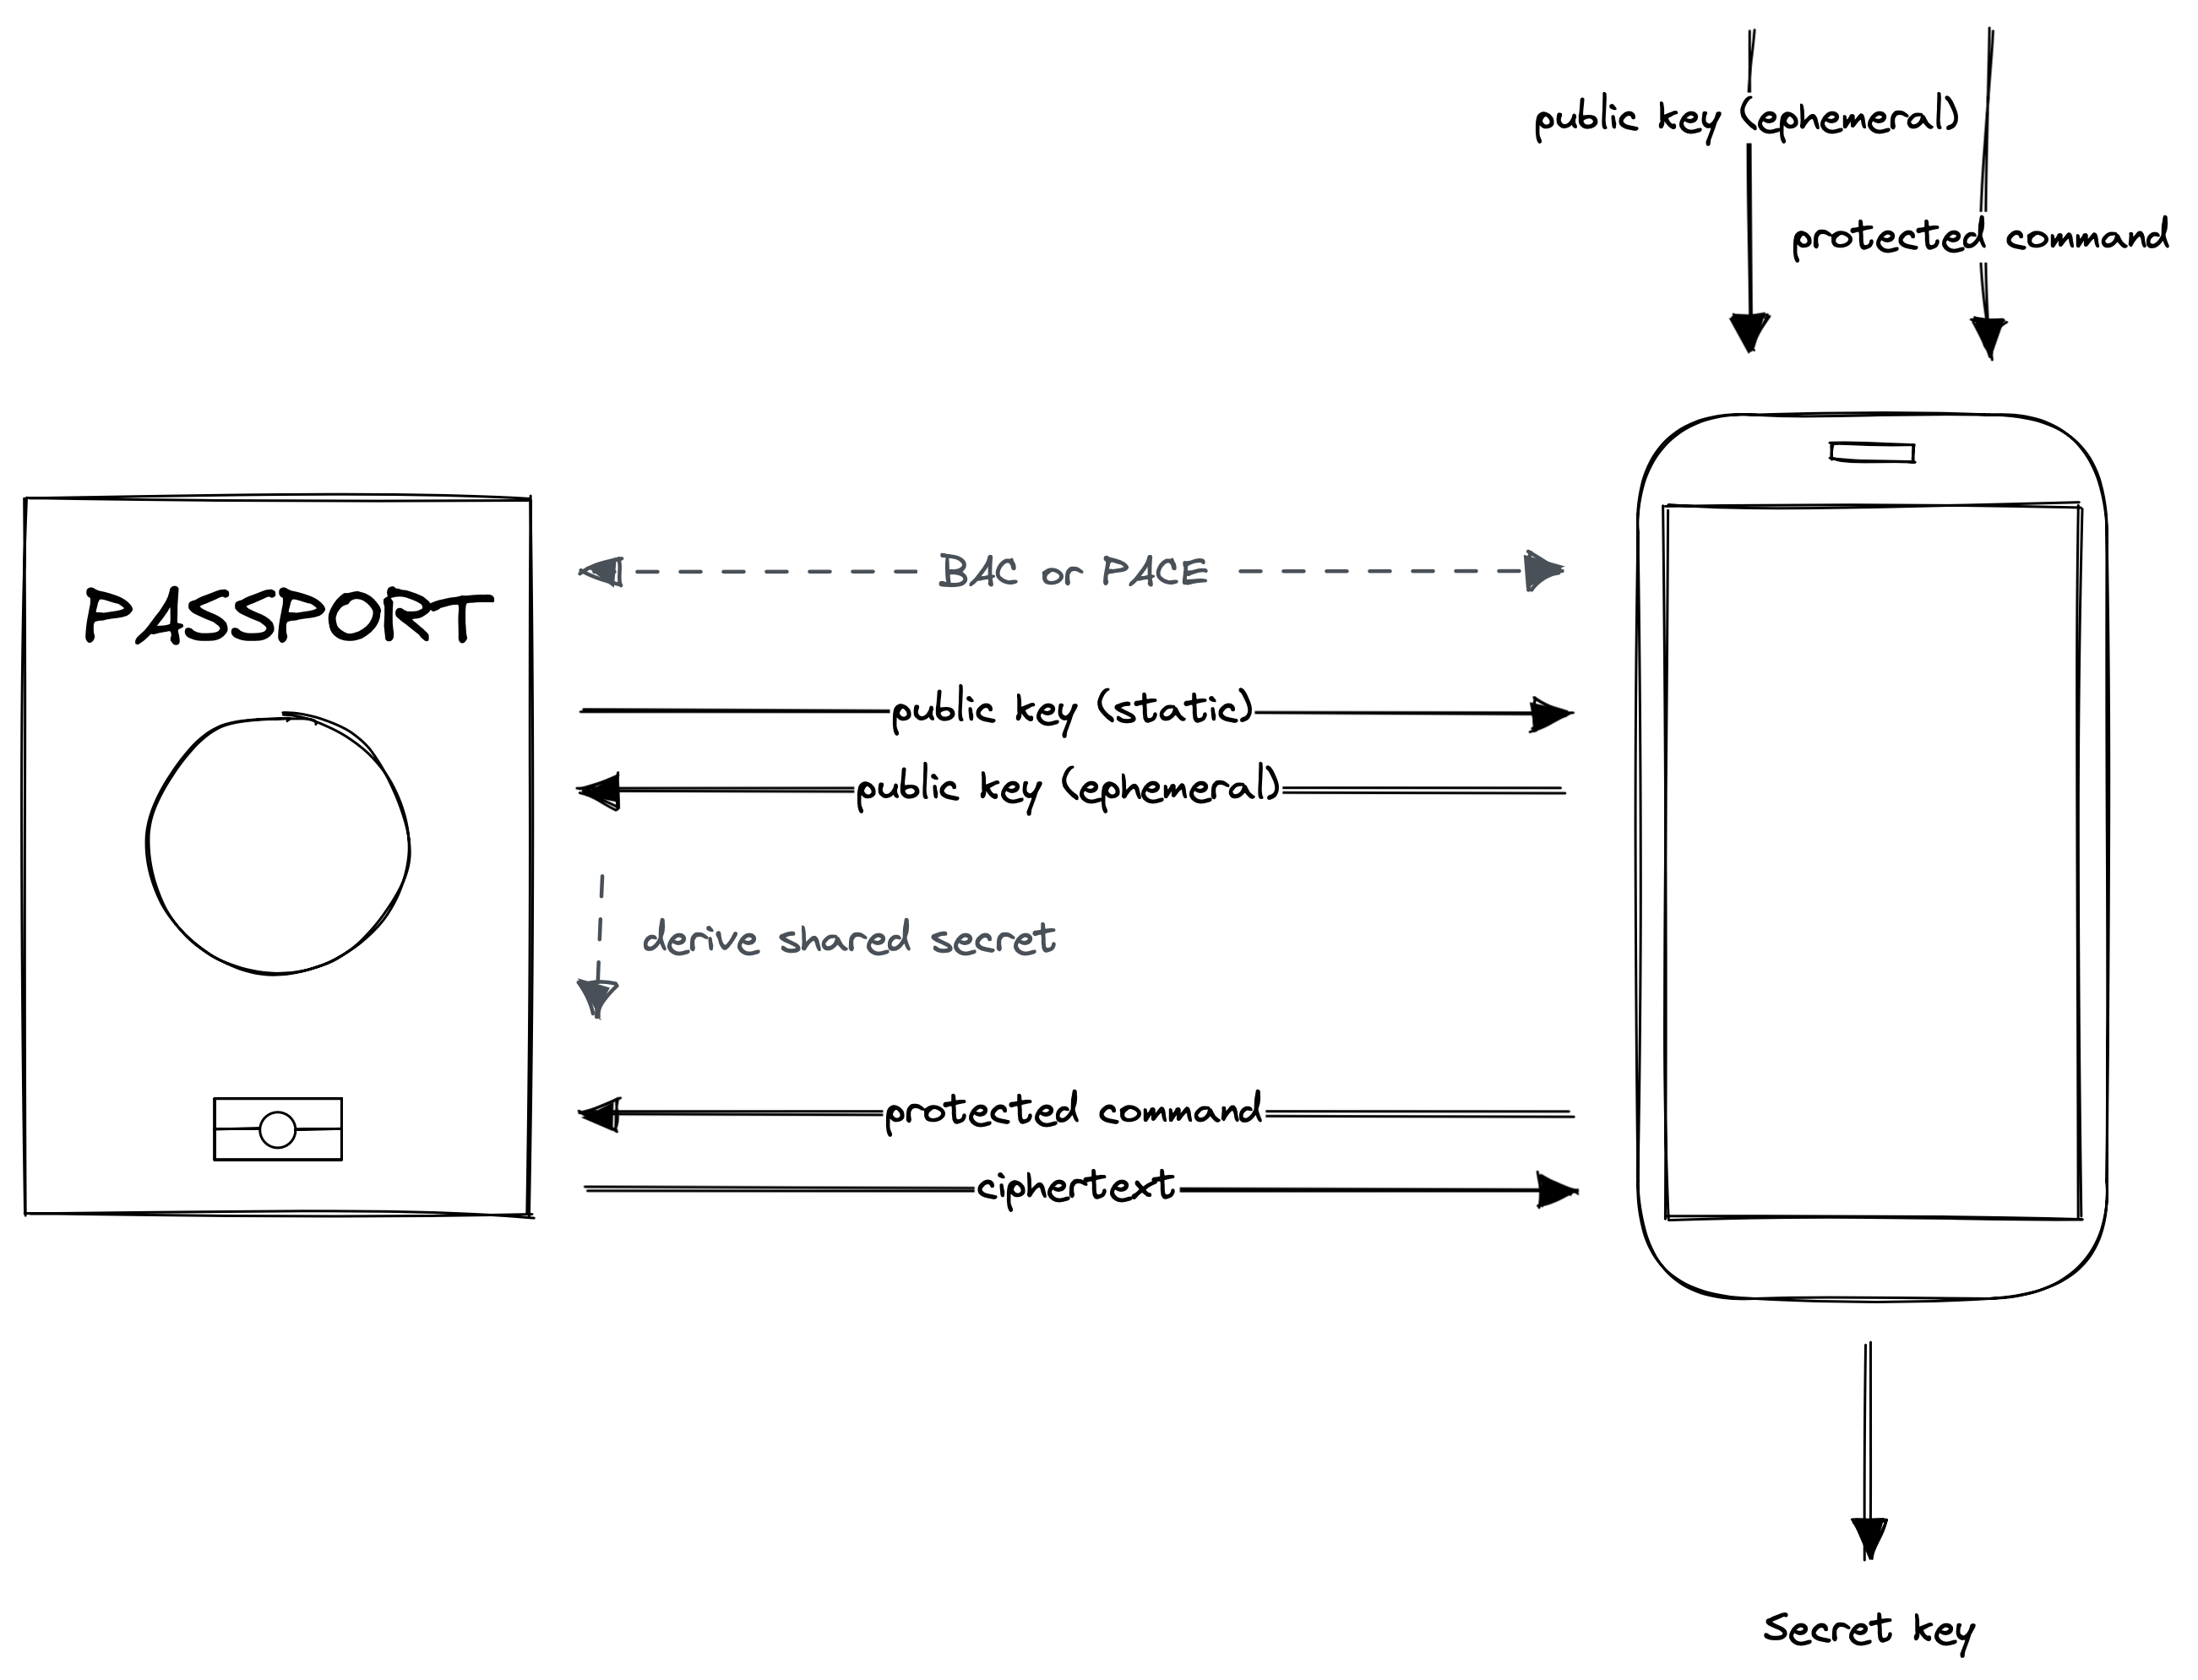
\includegraphics[width=0.8\linewidth]{imgs/RDE decryption}
    \caption{RDE decryption process}
    \label{fig:rde-decryption}
\end{figure}

\subsection{Trusting the reader}\label{subsec:trusting-the-reader}
We note that the reader itself does not store any secret information.
It only interfaces with the passport.
During the decryption (key retrieval) process, however, the reader will receive the secret key.
More importantly, the ciphertext that is used to derive the secret key is sent `in the clear' from the passport to the reader.
This means that not only the reader, but also anyone eavesdropping the communication between the reader and the passport can read this ciphertext.
For normal communication with the passport, BAC (though weak) or PACE offers protection against eavesdropping.
After CA, however, this protection is replaced.
For decryption, we thus need to trust the reader and the environment in which the reader is used.

\section{ICAO compatibility}\label{sec:icao-compatibility}
The RDE protocol relies on e-passports being able to perform Chip Authentication (CA) according to the ICAO standards~\cite{icao9303securitymechanisms}.
There are different key exchange protocols and cipher algorithms that can be used for CA.

The ICAO standard describes both standard RSA based Diffie-Hellman key agreement (DH) and ECDH based Diffie-Hellman key agreement (ECDH)~\cite{icao9303securitymechanisms}.
The standard also specifies that further communication should be encrypted using 112 bit 3DES in CBC mode, or 128-bit AES in CBC mode with CMAC, or 192-bit AES in CBC mode with CMAC or 256-bit AES in CBC mode with CMAC.
The standard does not restrict the use of specific curves for ECDH, meaning that any curve can be used.
However, it does specify a number of standard curves that can be used:
\begin{itemize}
    \item \texttt{brainpoolP192r1}
    \item \texttt{brainpoolP224r1}
    \item \texttt{brainpoolP256r1}
    \item \texttt{brainpoolP320r1}
    \item \texttt{brainpoolP384r1}
    \item \texttt{brainpoolP512r1}
    \item \texttt{secp192r1}
    \item \texttt{secp224r1}
    \item \texttt{secp256r1}
    \item \texttt{secp384r1}
    \item \texttt{secp521r1}
\end{itemize}
Any e-passport that is compliant with the ICAO standard on this level should be able to perform RDE.

As noted by Verheul in~\cite{verheul2017remote}, also other national ID cards and electronic drivers licenses that implement the ICAO CA(v1) standard should be able to perform RDE.
German identity cards, however, do not implement the ICAO CA v1 standard, but rather uses CA v2 that is not compatible with RDE because no static key from the passport is used in the key exchange.
Moreover, the German identity card requires the use of TA before reading any data group.

\section{Security}
\label{sec:security}
As described in~\cite{verheul2017remote}, the security of RDE is based on the security of the underlying CA protocol and the security of the encryption used for further communication.
For the Brainpool320r1 curve with 256-bit AES in CBC mode with CMAC, used on Dutch documents, RDE gives us 160-bit security.
Verheul does describe how longer ciphertexts can be achieved by not using a single protected command, but by using multiple protected commands, reading more bytes from data groups.
In this report, we do not go into the details of this, nor did we implement this, as the 160 bit security is already sufficient for our use case.
